\chapter*{Appendix}
\renewcommand{\thefigure}{A-\arabic{figure}}
\renewcommand{\thesection}{\Alph{section}}
\addcontentsline{toc}{chapter}{Appendix}
\section{Demonstration}
\subsection{HomePage}
\begin{figure}[H]
    \centering
    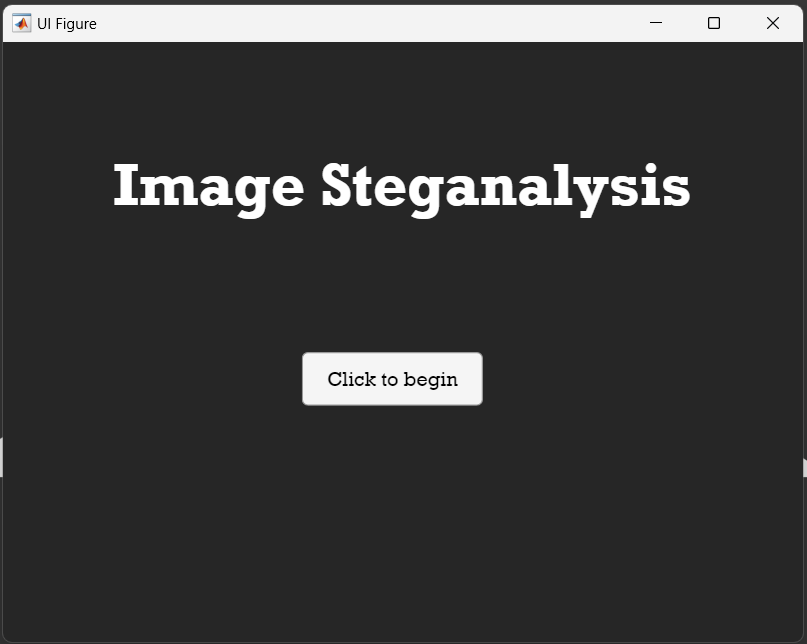
\includegraphics[width=140mm]{./img/HomePage.png}
    \caption{Home Page}
\end{figure}

\subsection{Image Upload Section}
\begin{figure}[H]
    \centering
    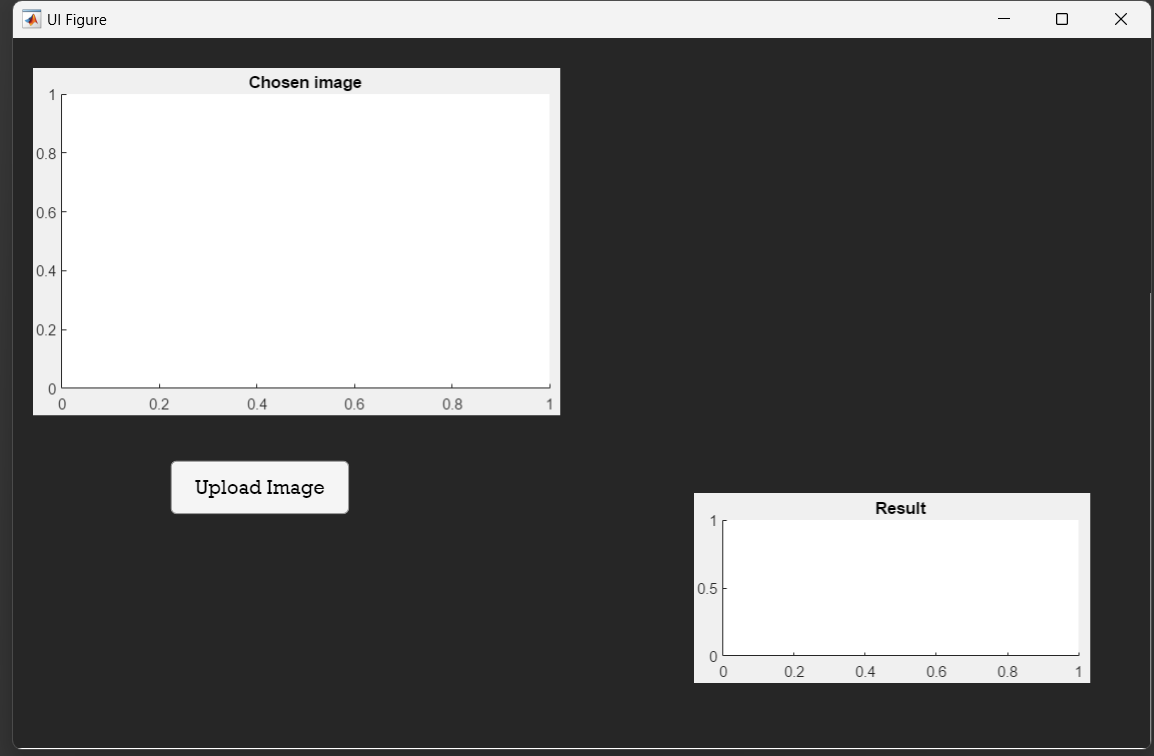
\includegraphics[width=140mm]{./img/choose.png}
    \caption{Image Upload Section}
\end{figure}

\subsection{Selection an Image}
\begin{figure}[H]
    \centering
    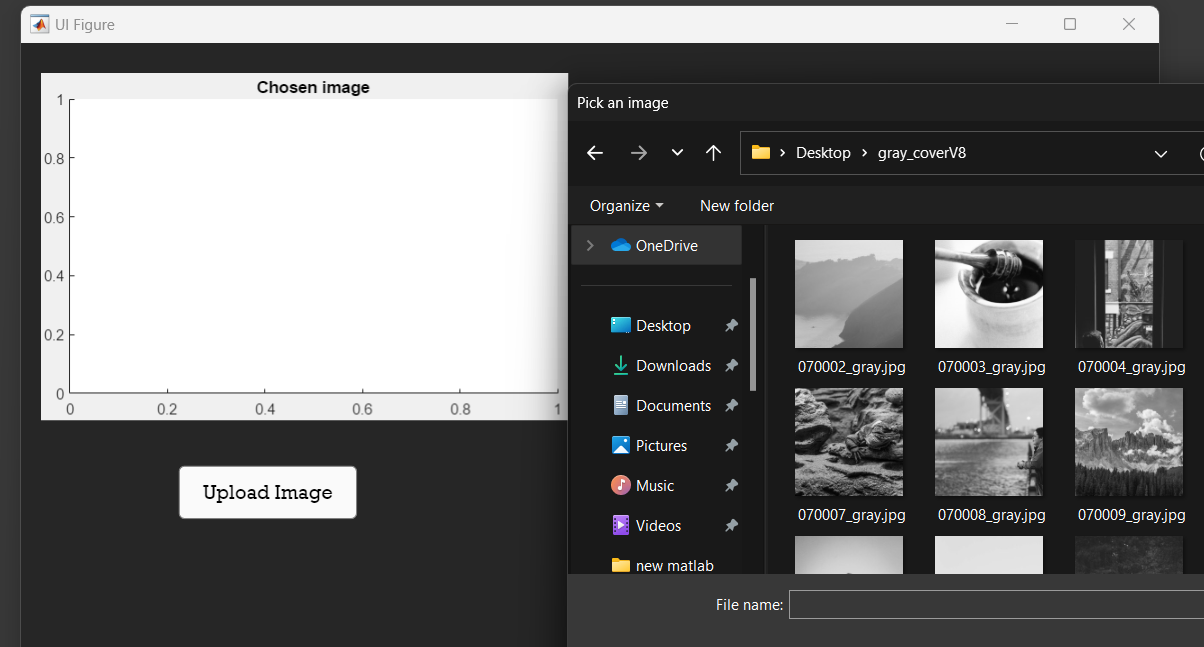
\includegraphics[width=140mm]{./img/selectsample.png}
    \caption{Image Selection}
\end{figure}

\subsection{Results}
\begin{figure}[H]
    \centering
    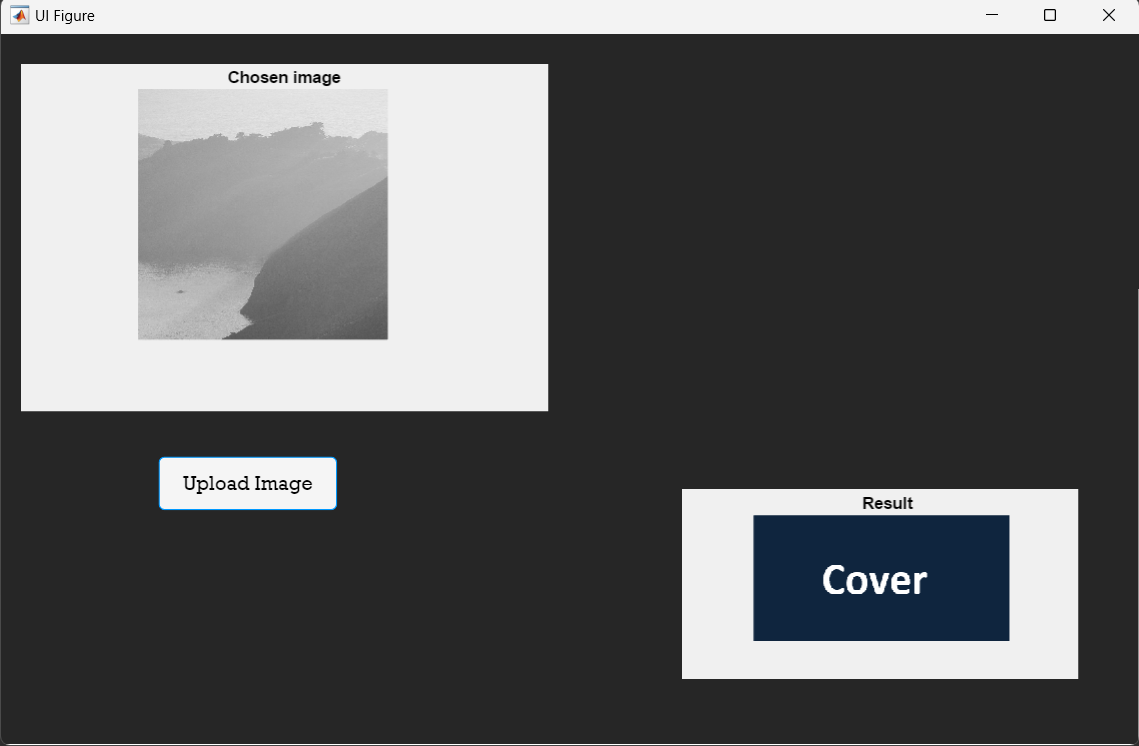
\includegraphics[width=140mm]{./img/resultGrayCover.png}
    \caption{Result}
\end{figure}
\begin{figure}[H]
    \centering
    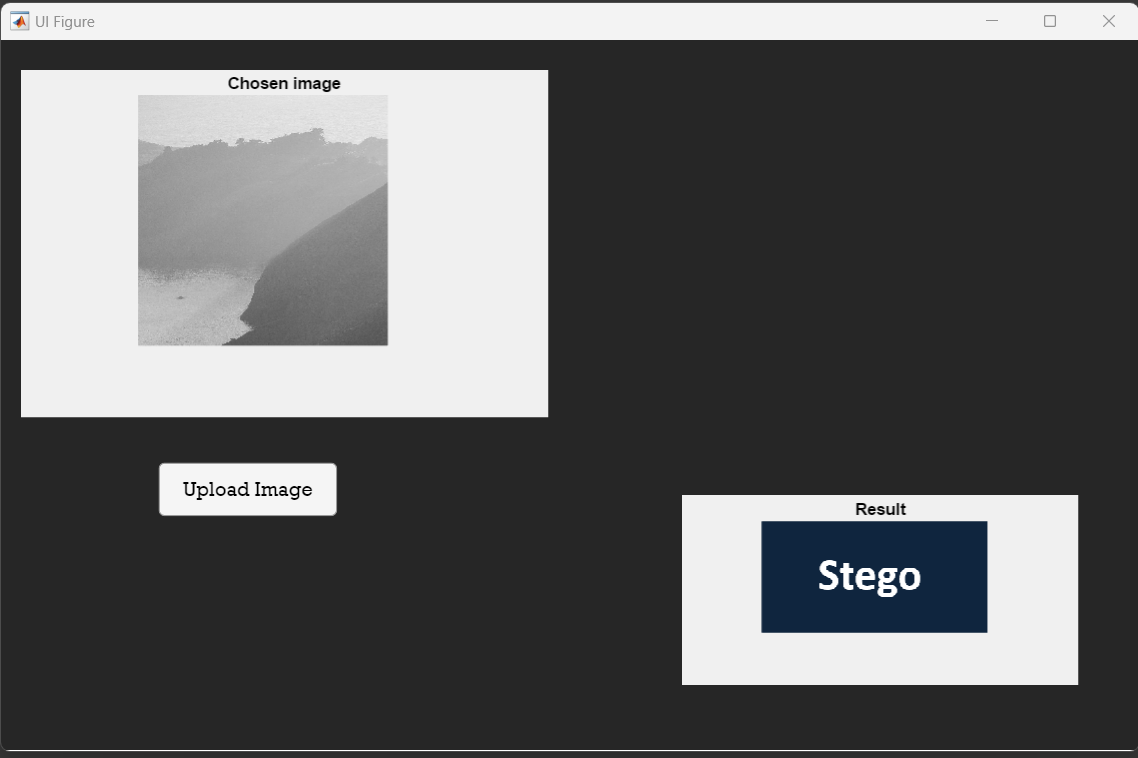
\includegraphics[width=140mm]{./img/resultGrayStego.png}
    \caption{Result}
\end{figure}

\section{Model Training}
\subsection{Splitting Dataset}
\begin{figure}[H]
    \centering
    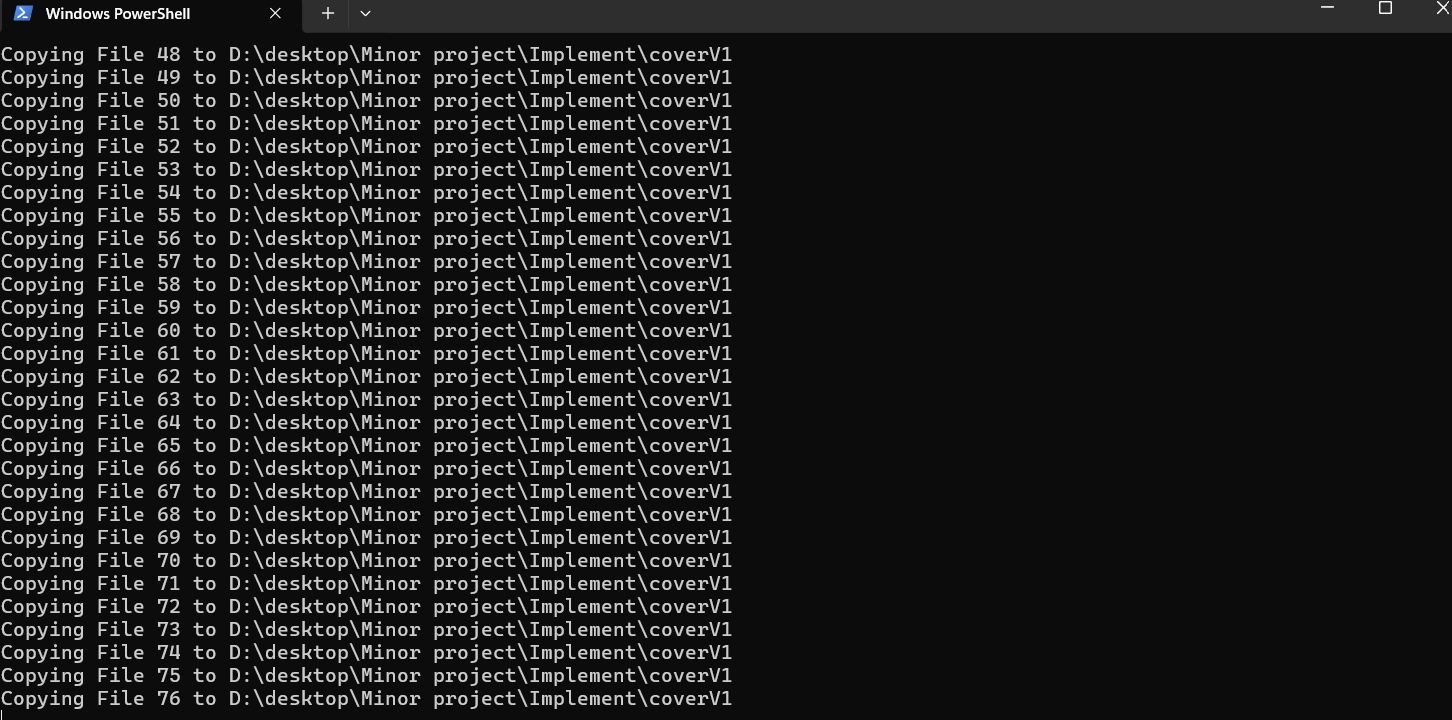
\includegraphics[width=150mm]{./img/splitting.png}
    \caption{Splitting Dataset using PowerShell Script}
\end{figure}
\subsection{Feature Extraction}
\begin{figure}[H]
    \centering
    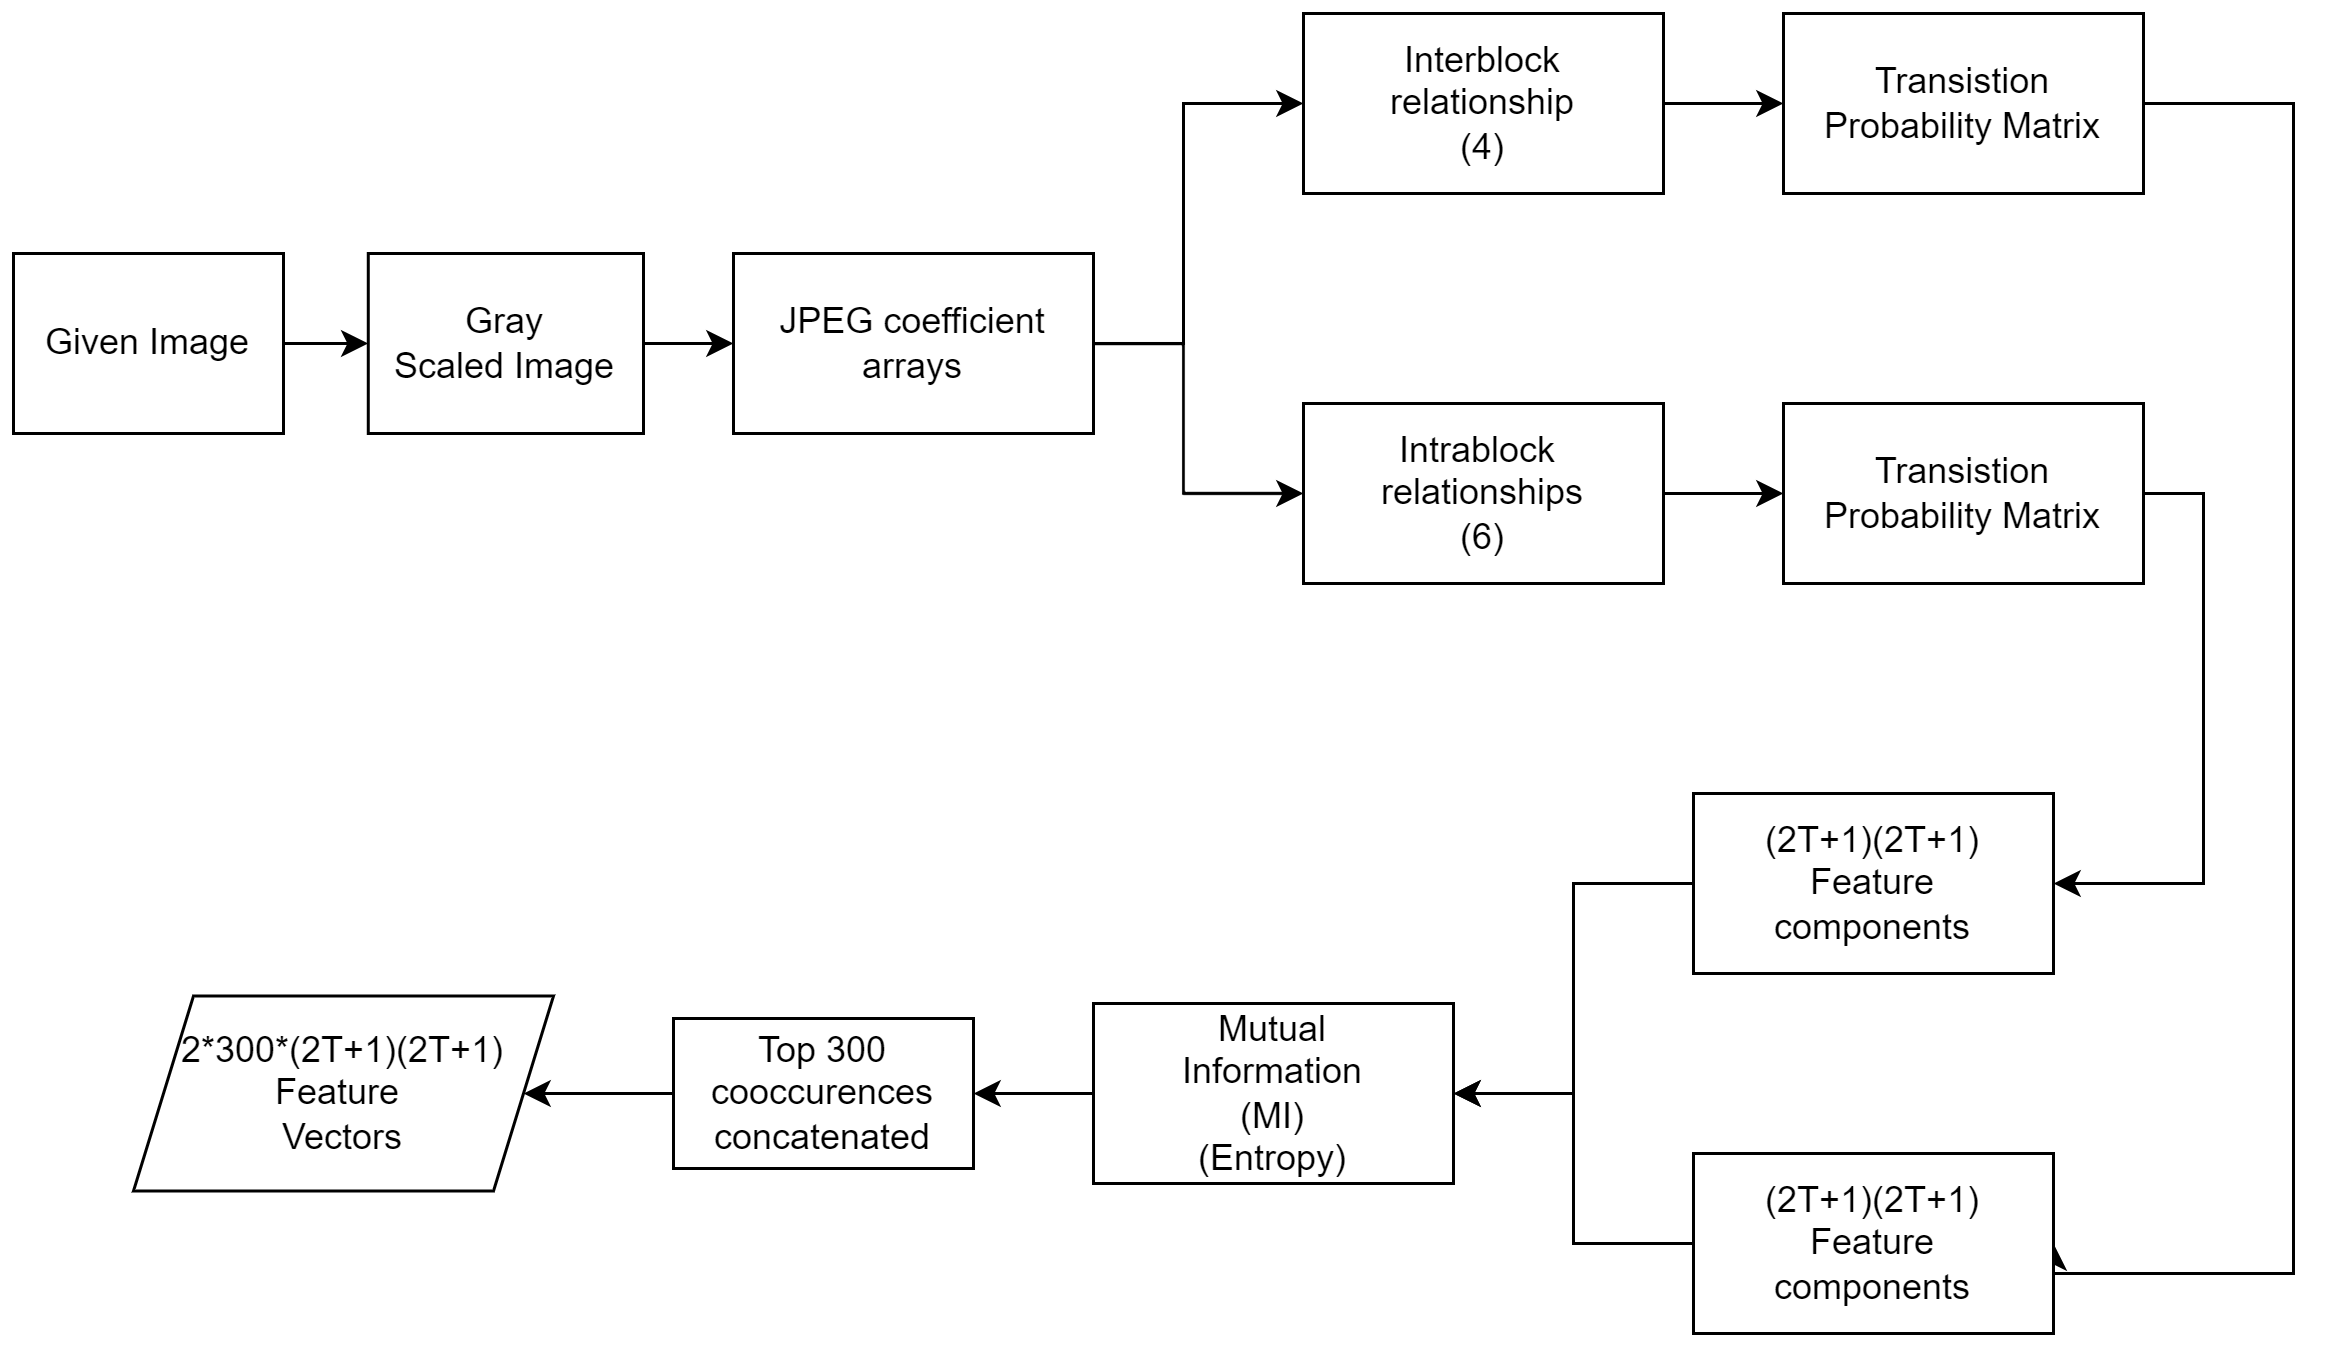
\includegraphics[width=150mm]{./img/feature_extraction.png}
    \caption{Feature Extraction Screenshot}
\end{figure}
\subsection{Model Training}
\begin{figure}[H]
    \centering
    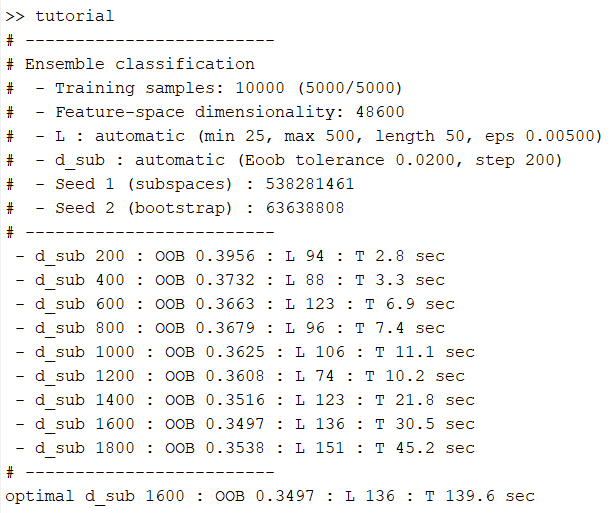
\includegraphics[width=150mm]{./img/training.png}
    \caption{Model Training Screenshot}
\end{figure}